\documentclass[12pt]{beamer}
\usetheme{CambridgeUS}
\usecolortheme{dolphin}
\usepackage[utf8]{inputenc}
\usepackage{amsmath}
\usepackage{amsfonts}
\usepackage{amssymb}
\usepackage{graphicx}
\usepackage{mathtools}
\usepackage{multimedia}
\usepackage[mathscr]{euscript}
\usepackage{xcolor}
\usepackage{algorithmicx}
\usepackage{algpseudocode}
\usepackage{setspace}
\usepackage[overlay,absolute]{textpos}

\DeclarePairedDelimiter{\abs}{\lvert}{\rvert}
\DeclarePairedDelimiter{\norm}{\lVert}{\rVert}

\newcommand{\R}{\mathbb{R}}
\newcommand{\C}{\mathbb{C}}
\newcommand{\Tau}{\mathcal{T}}
\newcommand{\AMz}{\underset{z}{arg\, min}}
\newcommand{\prox}{\text{prox}}

\newcommand{\worm}{WWWWWoooooooRRRRRmmmmmm}

\author[Rudy,Maass,Molloy,Mueller]{Samuel Rudy, Kelsey Maass, Riley Molloy, and Kevin Mueller}
\title[Denoising and Deblurring]{Image Denoising and Deblurring \\ \normalsize Applied Math 515 Final Project}
\setbeamercovered{transparent} 
%\institute{University of Washington} 
\date{March 12 2016} 
\subject{Amath 575} 

\iffalse
To d:
-Discuss different fidelity functions
-Discuss different regularizers
-Talk about optimization for wavelet method
-Talk about Frobenius norm denoising
-TV reg for denoising and deblurring
-Give lots of examples
-Talk about caveats of each method (parameters are a pain in the ass)
-bibliography
\fi

\begin{document}

% Title Page
\begin{frame}
\titlepage
\end{frame}

% Contents
\begin{frame}{Contents}
\tableofcontents
\end{frame}

% MOTIVATION
\section{Motivation}

% Cameraman example
\begin{frame}{Image Denoising and Deblurring}
\begin{center}
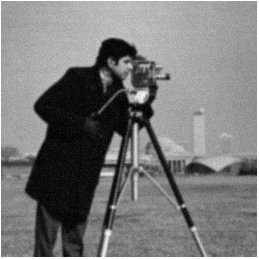
\includegraphics[scale=0.55]{../figures/bad_image.png}
\hspace{1 cm}
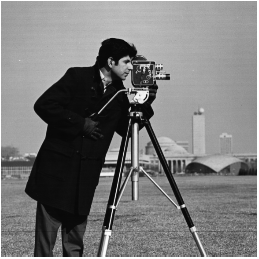
\includegraphics[scale=0.55]{../figures/good_image.png} 
\end{center}
\end{frame}

% Problem Formulation
\begin{frame}{Mathematical Formulation}
\begin{center}
\vspace{-3ex}
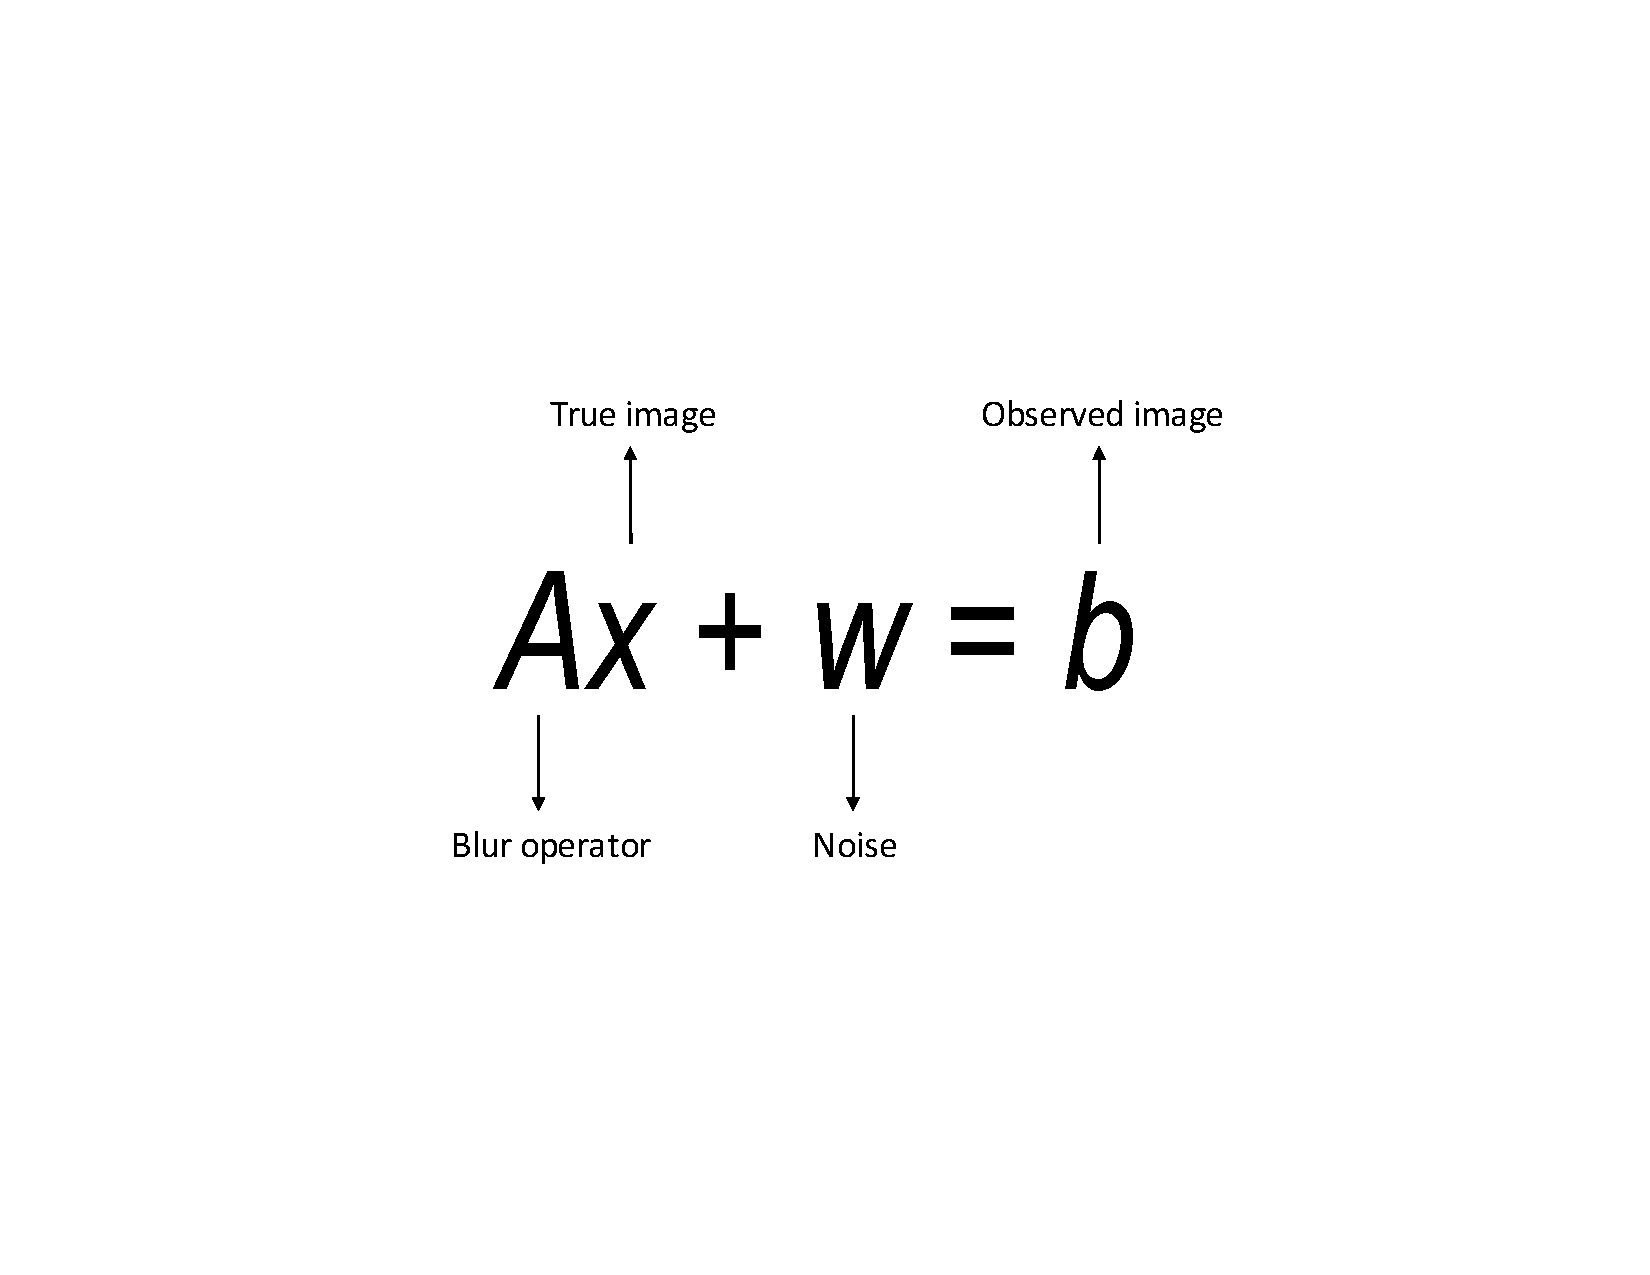
\includegraphics[scale=0.5]{../figures/linearModel}
\end{center}

\vspace{-3ex}
\begin{itemize}
\item Blur: $Ax$ is a discrete convolution of the true image with a Gaussian kernel (reflexive boundary conditions).
\item Noise: $w$ is noise drawn from a Gaussian or Student's t distribution. 
\end{itemize}
\end{frame}

% Naive Solution
\begin{frame}{Naive Solution: $x = A^{-1}b$}
\begin{figure}
\centering
%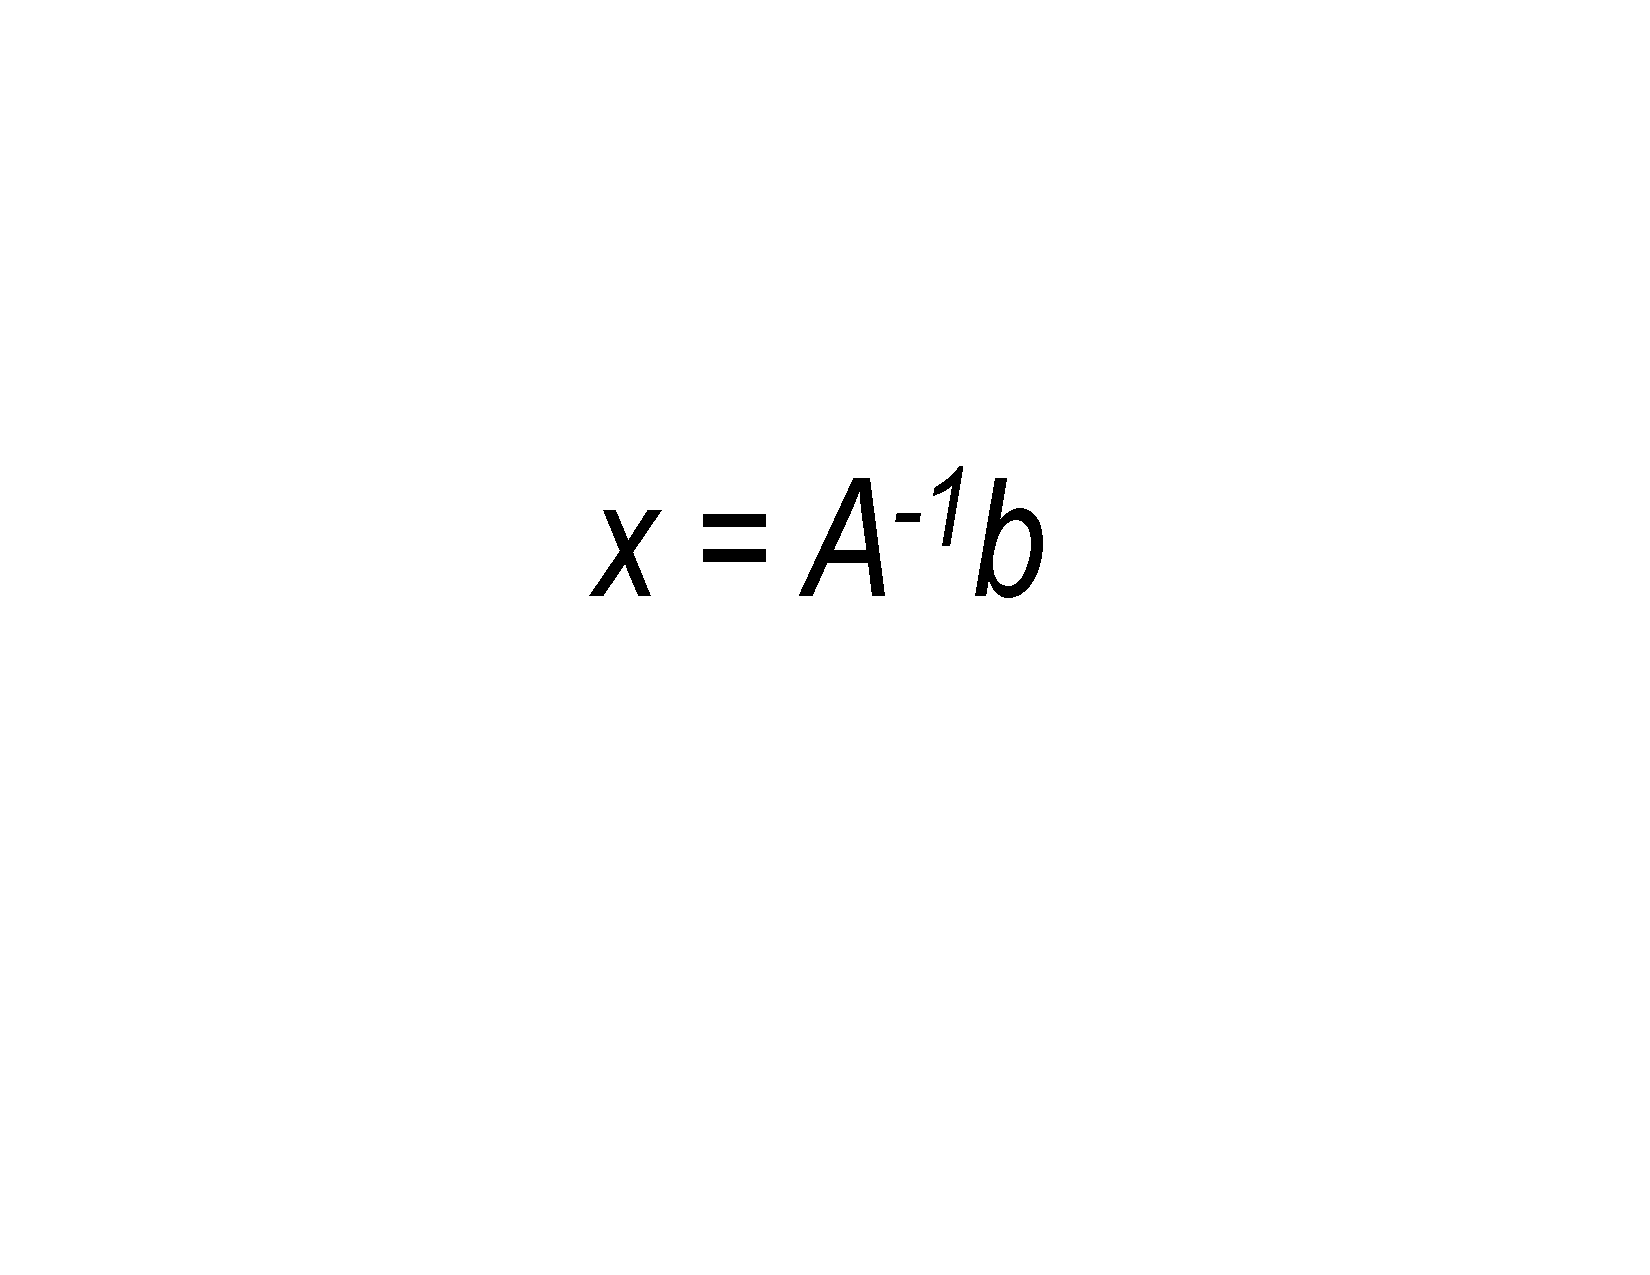
\includegraphics[scale=0.4]{../figures/naive1} \\[2ex]
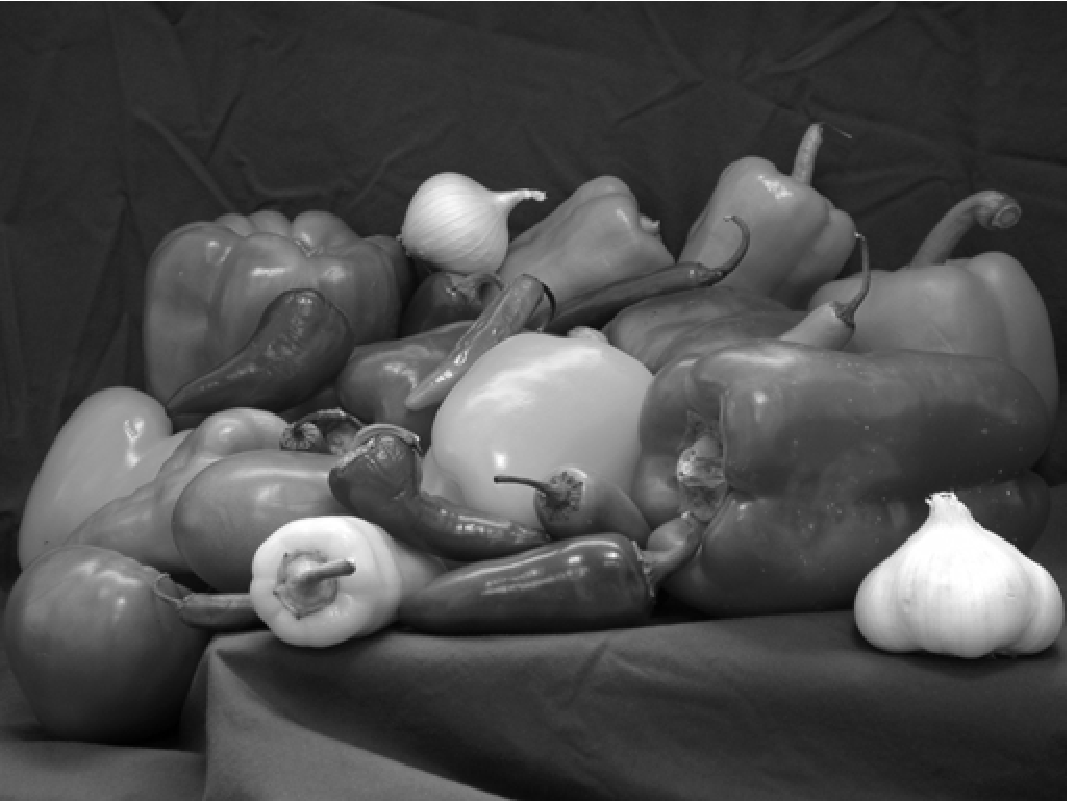
\includegraphics[scale=0.2]{../figures/fig1} \,
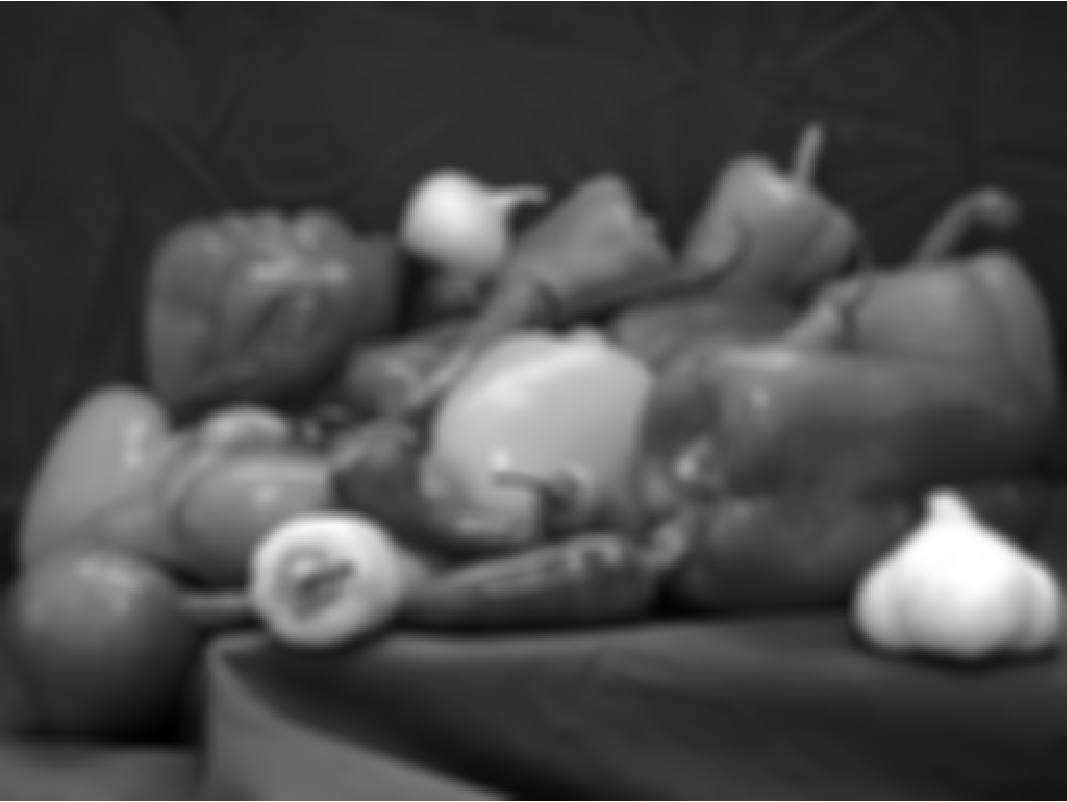
\includegraphics[scale=0.2]{../figures/fig2} \,
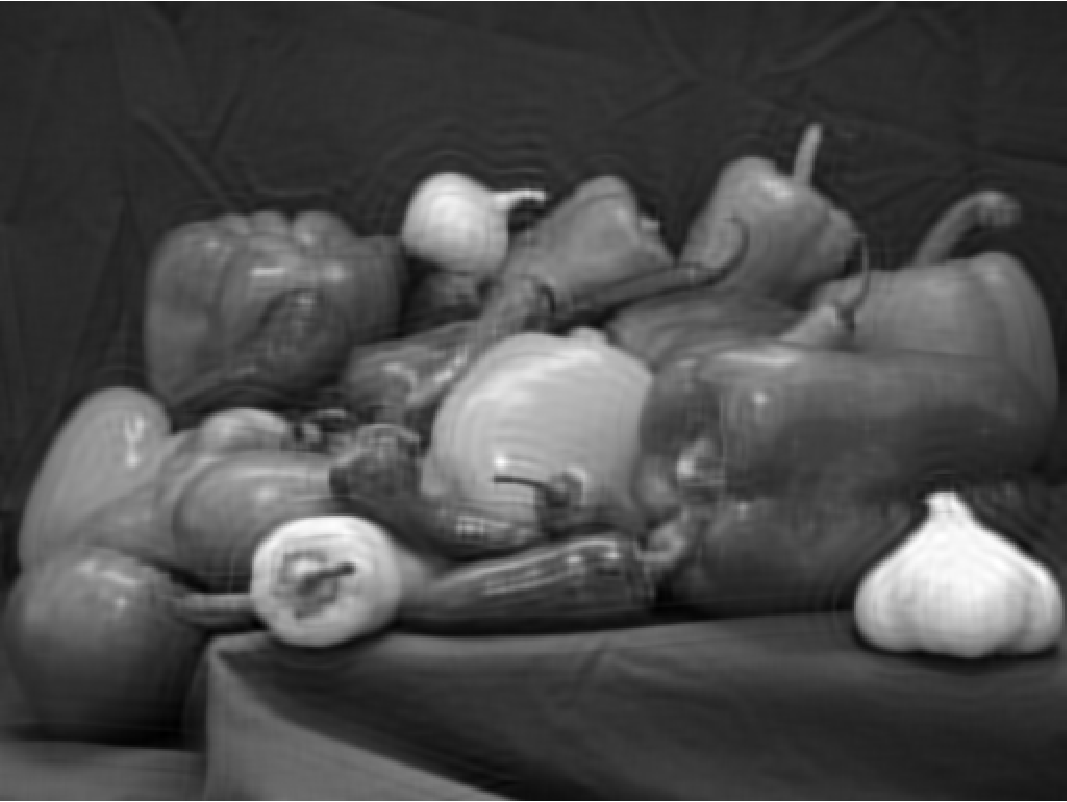
\includegraphics[scale=0.2]{../figures/fig3} \\
\small{\hspace{1em} True image \hspace{4em} Blurred image \hspace{3em} Recovered image}
\end{figure}
\end{frame}

\begin{frame}{Naive Solution: $x = A^{-1}(b-w)$}
\begin{figure}
\centering
%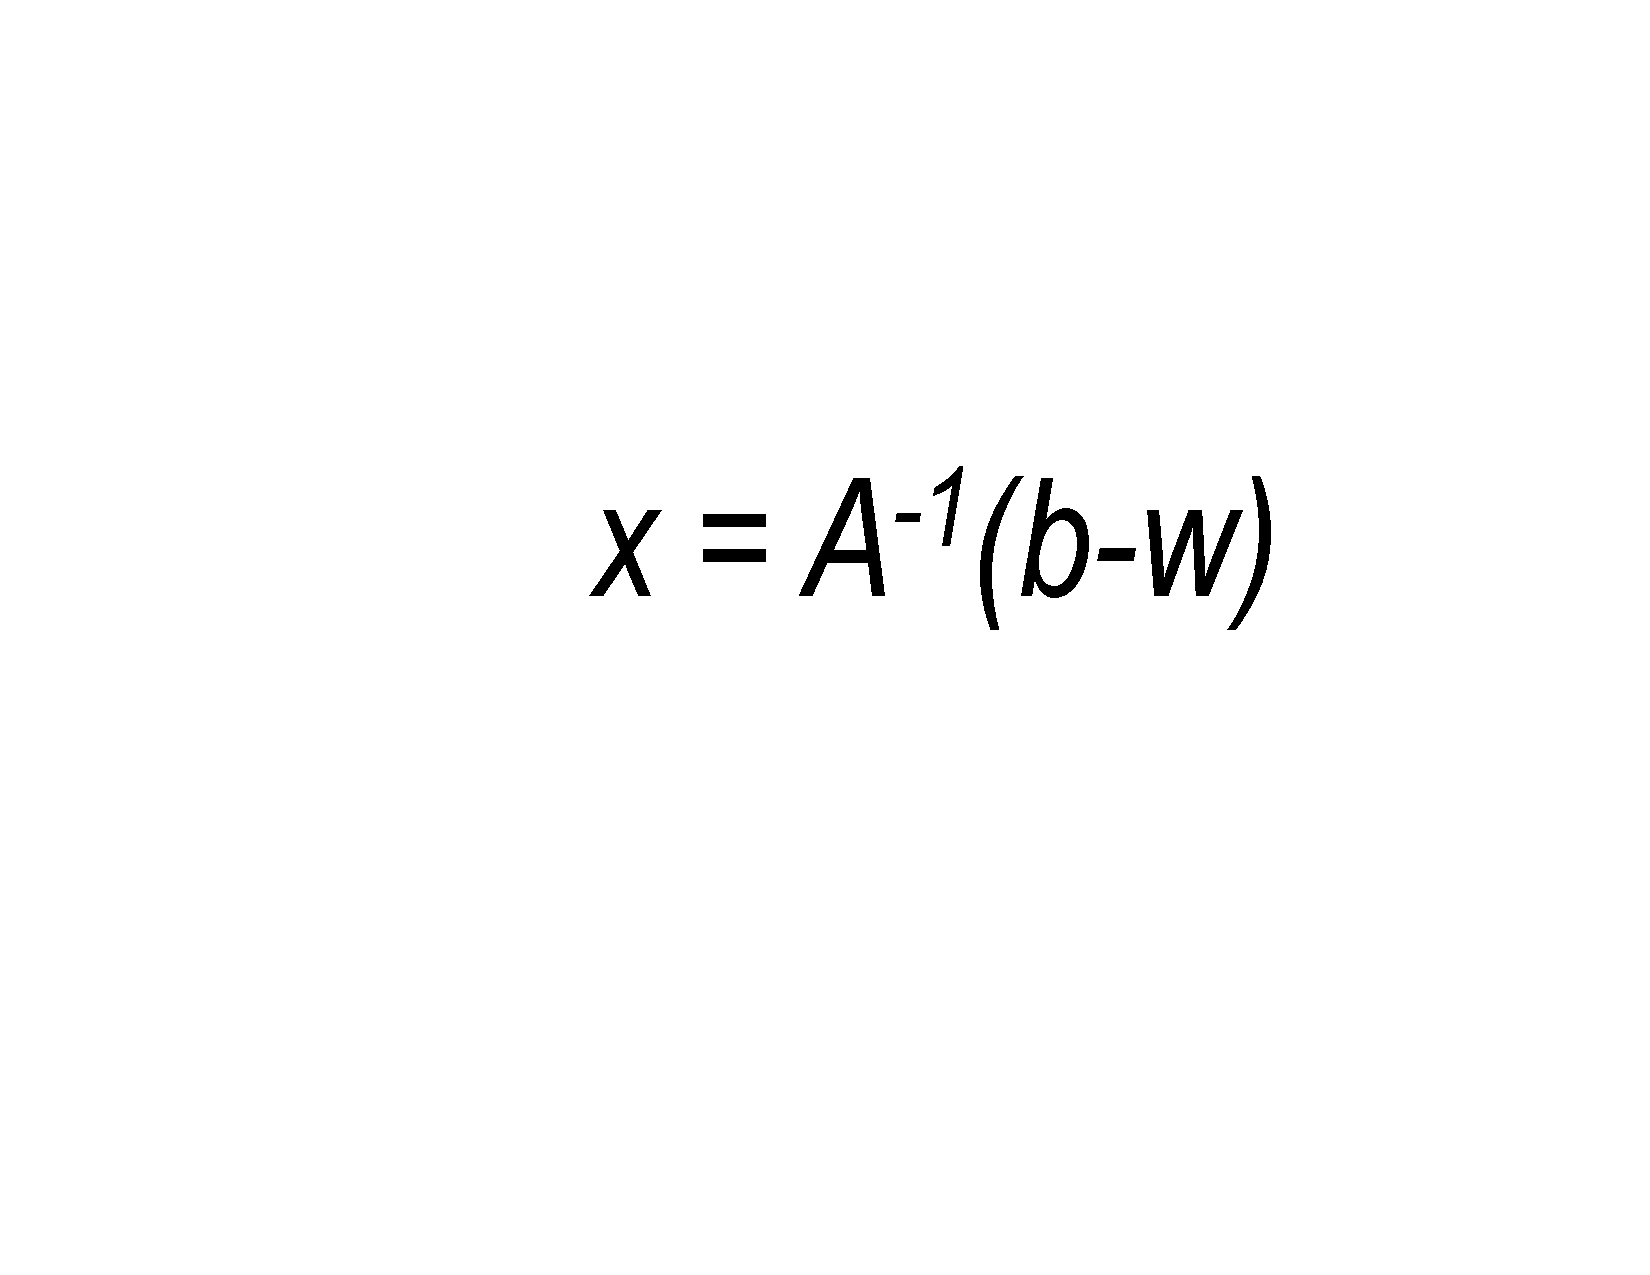
\includegraphics[scale=0.4]{../figures/naive2} \\[2ex]
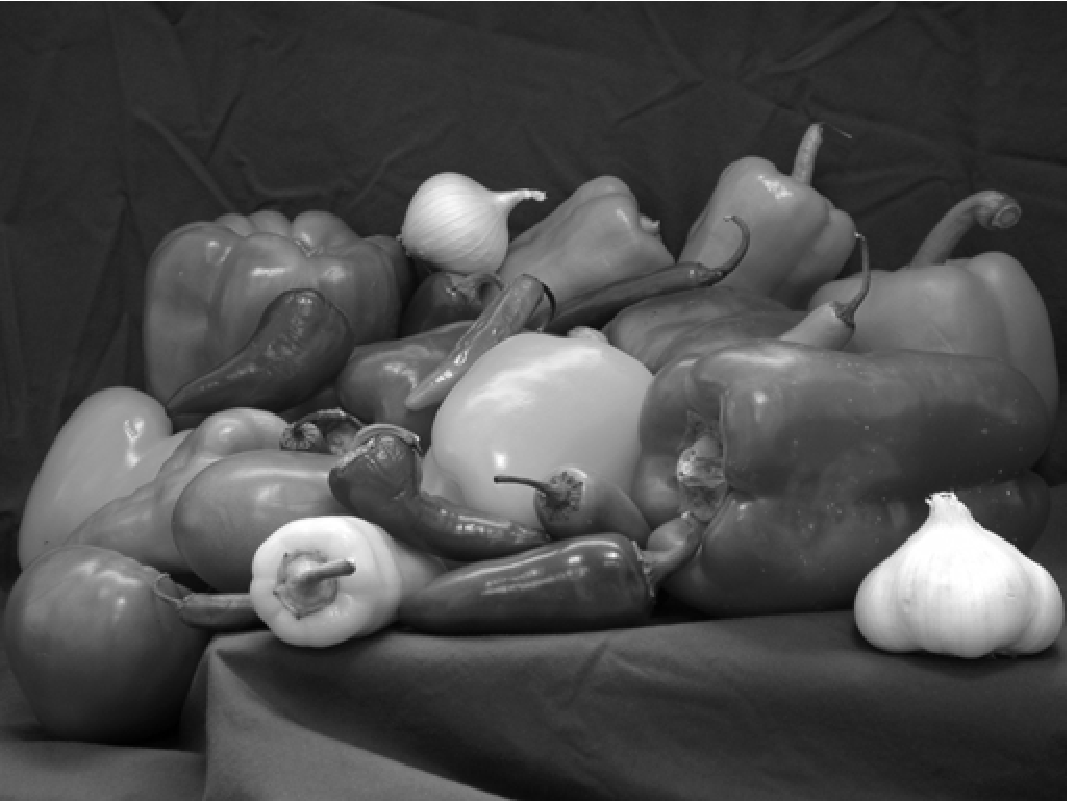
\includegraphics[scale=0.2]{../figures/fig1} \,
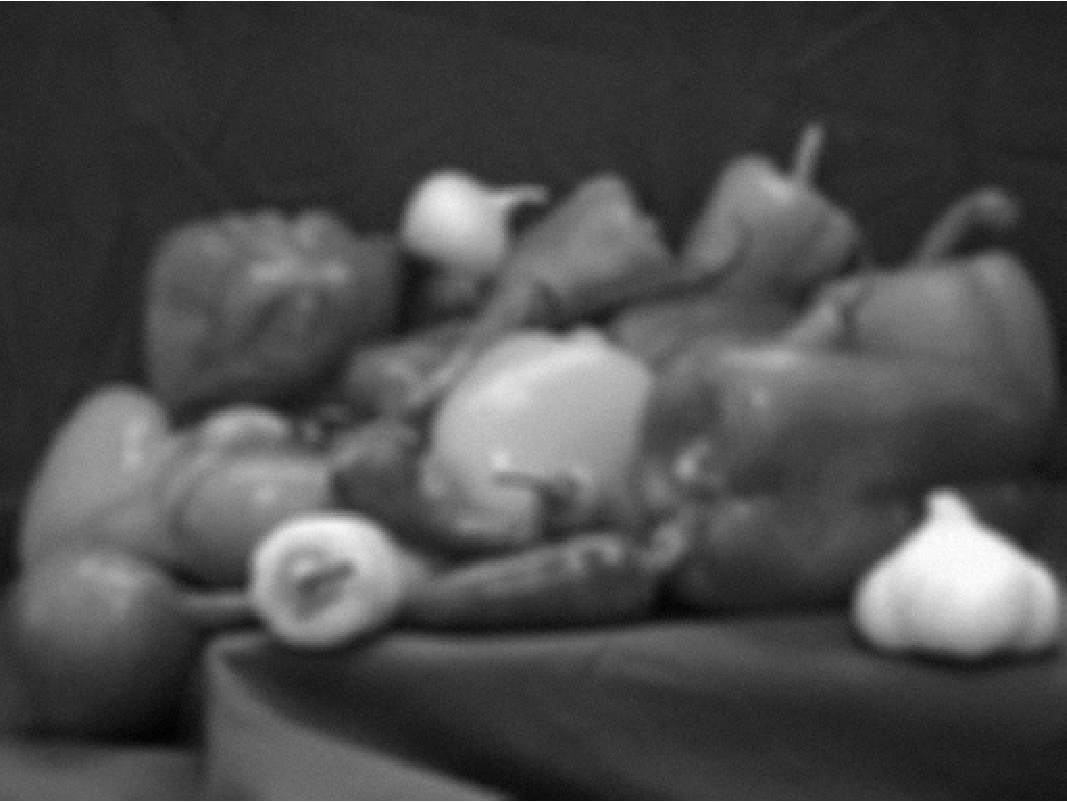
\includegraphics[scale=0.2]{../figures/fig4} \,
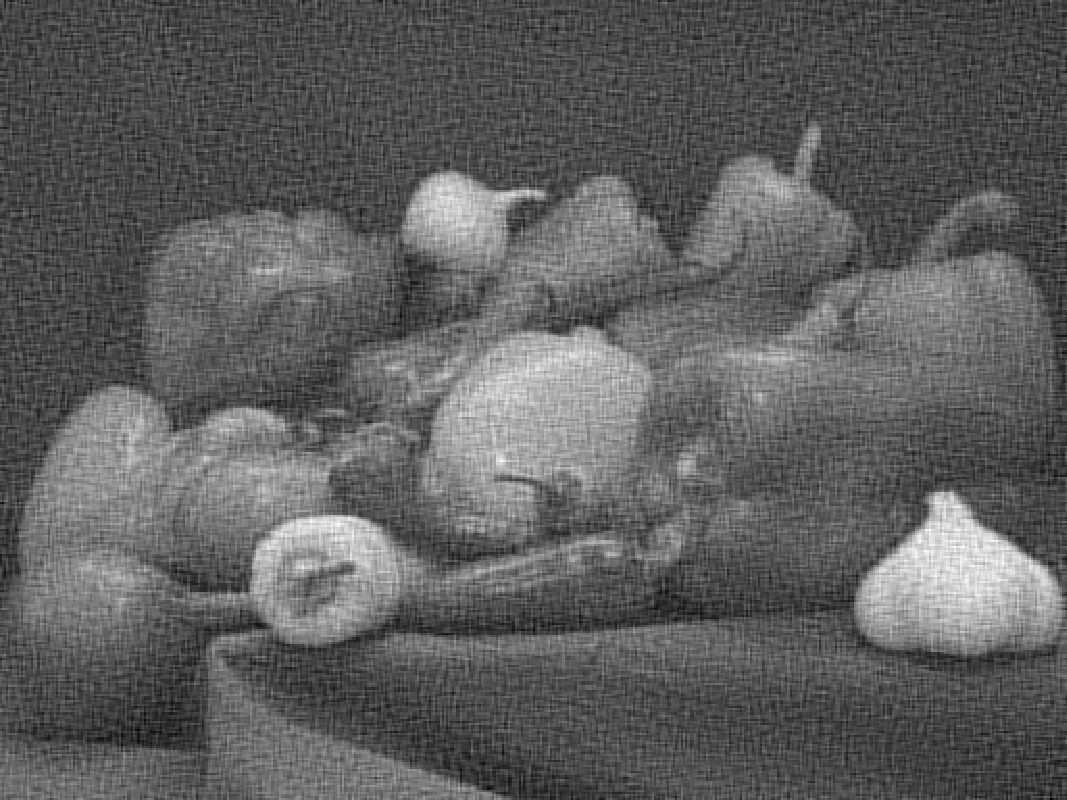
\includegraphics[scale=0.2]{../figures/fig5} \\
\small{\hspace{1em} True image \hspace{2em} Blurred and noisy image \hspace{1em} Recovered image}
\end{figure}
\end{frame}

% OBJECTIVE FUNCTIONS
\section{De(noise/blur)ing Objective Functions}

% General Loss Function
\begin{frame}
Since the blur operator is ill-conditioned, a better approach is to minimize a regularized loss function.
\begin{block}{General Loss Function}
\[ L_b(x) \hspace{0.5em} = \hspace{0.5em} \underbrace{f(Ax-b)}_{\text{Fidelity term}} \hspace{0.5em} + \underbrace{\lambda R(x)}_{\text{Regularization}} \]
\end{block}

\begin{columns}[T]
	\begin{column}{0.45\linewidth}
		\begin{block}{Fidelity Terms} \vspace{-2.5ex}
			\[ f = \left\{ \begin{matrix*}[l] 
			\| \cdot \|_F^2 \\[1ex] h_{\gamma}( \cdot ) \\[1ex] \gamma^{-1} \log(\cosh(\gamma \cdot)) 
			\end{matrix*} \right. \]
		\end{block}
	\end{column}
	\begin{column}{0.45\linewidth}
		\begin{block}{Regularization Terms}
			\[ R = \left\{ \begin{matrix*}[l]
			\| Wx \|_1 \\[1ex] TV(x)
			\end{matrix*} \right. \]
		\end{block}
	\end{column}
\end{columns}
\end{frame}

% Fidelity Term
\begin{frame}{Fidelity Term Penalty Functions}

The fidelity term $f(Ax-b)$ measures how well our results comply with the linear blurring model. Depending upon the type of noise present in the observed image, the choice of penalty function may influence the efficacy of our deblurring/denoising procedure. 

\begin{columns}[T]
	\begin{column}{0.45\linewidth}
		\begin{block}{Gaussian Noise}
		\quad 
\includegraphics[scale=0.15]{../figures/gaussian_noise.png} \hspace{1.5em}
		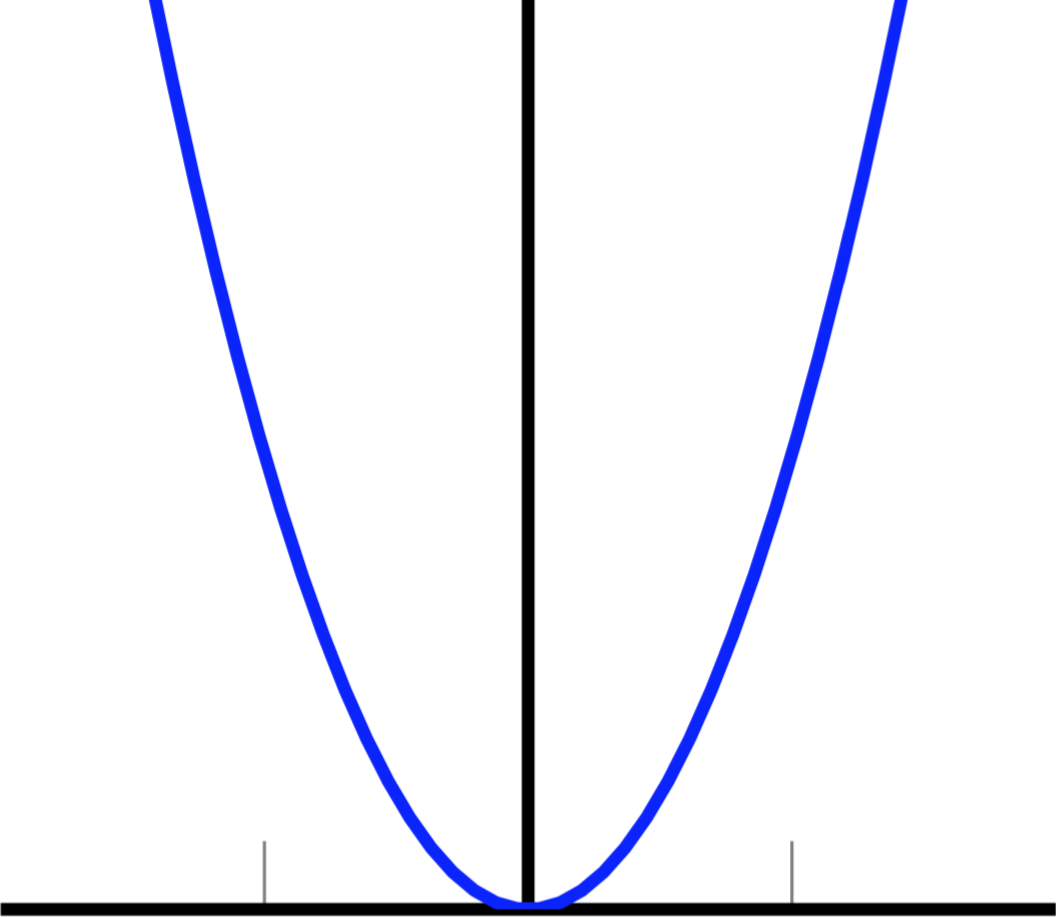
\includegraphics[scale=0.1]{../figures/quadratic} \\
		{\footnotesize Due to the lack of outliers, the quadratic penalty is sufficient} \\[1ex]
		\hspace{3em} $f(z) = \frac{1}{2} \| z \|^2$
		\end{block}
	\end{column}
	\begin{column}{0.45\linewidth}
		\begin{block}{Student's t Noise}
		\quad 
\includegraphics[scale=0.15]{../figures/student_t_noise.png} \hspace{1.5em}
		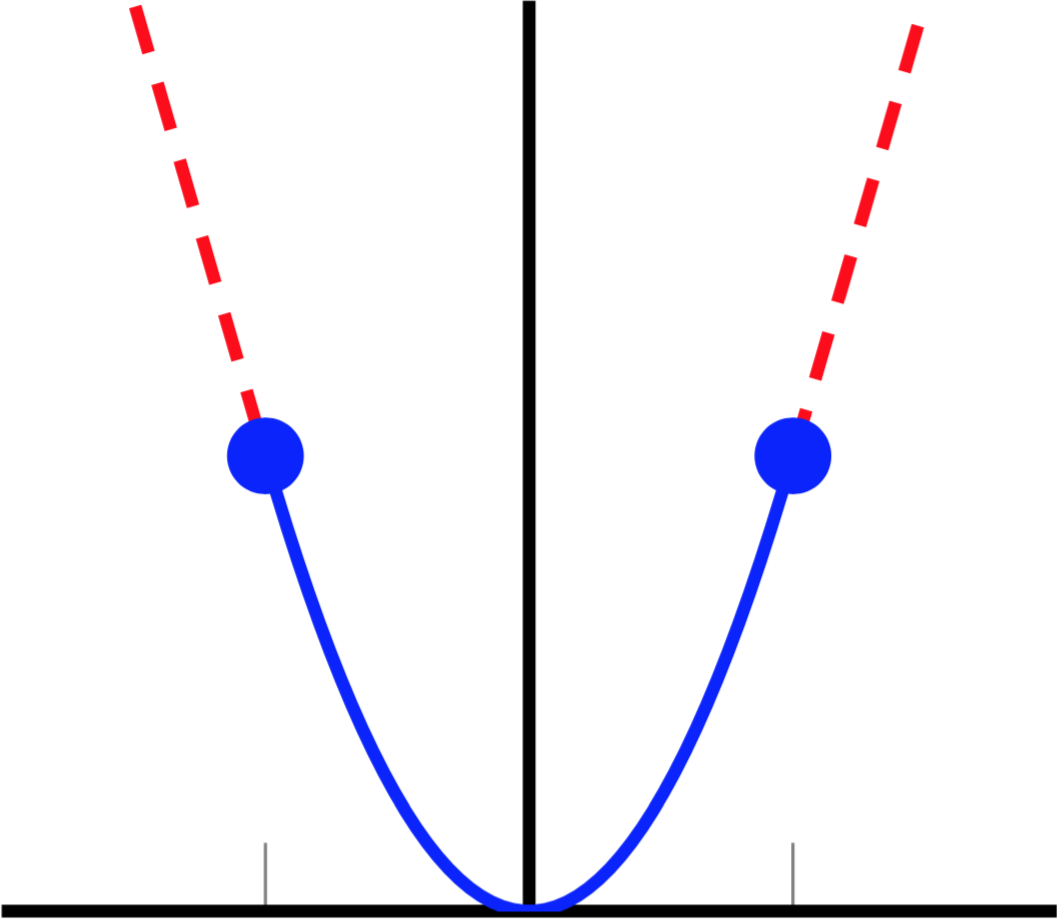
\includegraphics[scale=0.1]{../figures/huber} \\
		{\footnotesize Huber penalty preferred since it is more robust to heavy-tailed noise} \\[1ex]
		$f(z) = \min_y \frac{1}{2} \| z-y \|^2 + \gamma \| y \|_1$
		\end{block}
	\end{column}
\end{columns}

\end{frame}

% Regularizers
\begin{frame}{Image Assumptions and Regularizers}

\begin{textblock}{6}(2,3.2)
2-Level Haar Transform
\end{textblock}

\begin{textblock}{6}(8.7,3)
$|x_{ij} - x_{i+1,\,j}| + |x_{ij}-x_{i,\,j+1}|$ 
\end{textblock}

\begin{center}
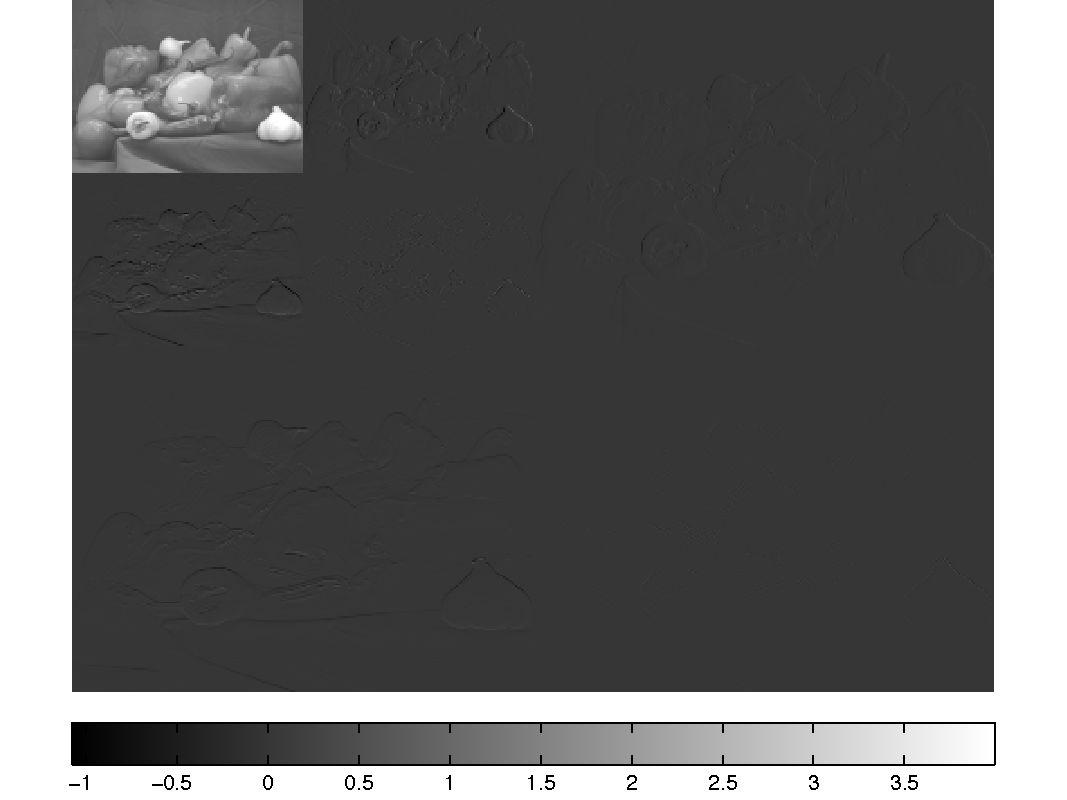
\includegraphics[width=0.5\linewidth]{../figures/haarTrans.pdf} \hspace{-1em}
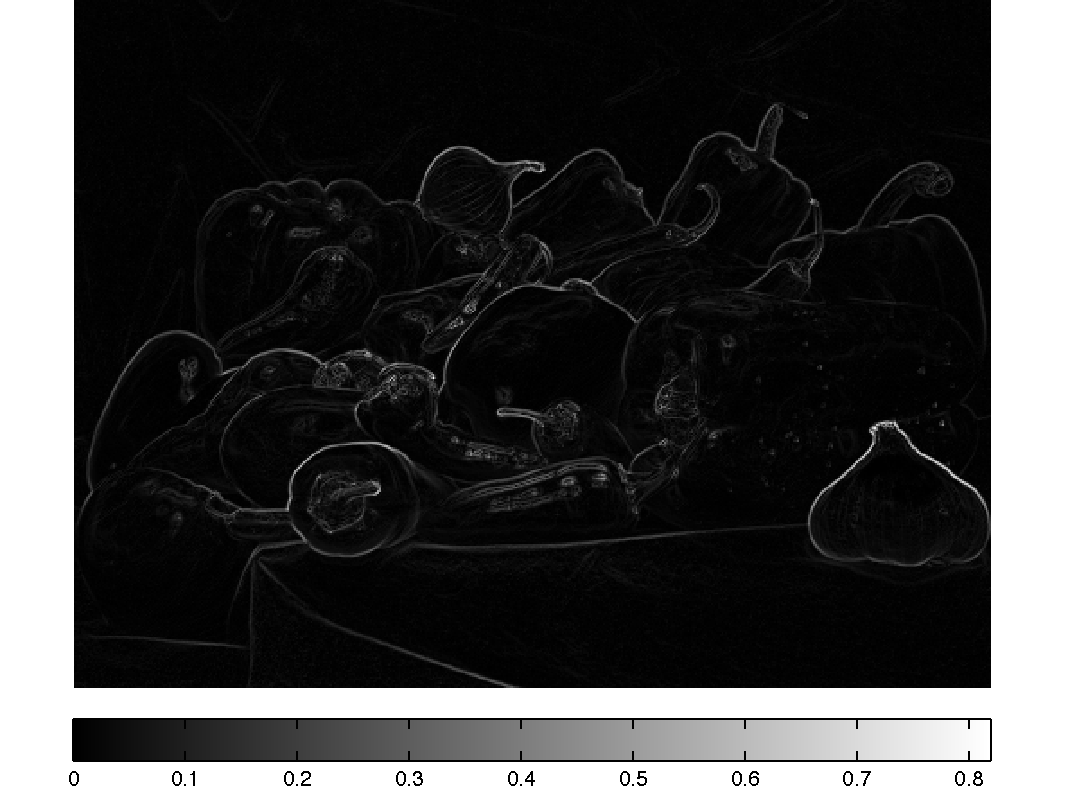
\includegraphics[width=0.5\linewidth]{../figures/diff.pdf}
\end{center}

Our choices of regularizers assume that images are sparse in wavelet domains and that they are relatively smooth (low total variation).
SPLIT THIS INTO 2 SLIDES

% Talk about choice of R
% Haar, FFT
% What is TV?
% Show two different definitions of TV from paper.

%%%%%%%%%%%%%%%%%%%%%%%%%%%%%%%%%%%%%%%%%%%%%%%%%
% We could split this up into two slides so that we can have a little more info on each regularizer. 
%%%%%%%%%%%%%%%%%%%%%%%%%%%%%%%%%%%%%%%%%%%%%%%%%

\end{frame}

% OPTIMIZATION WITH L1 WAVELET REGULARIZATION
\section{Optimization with L1 Wavelet Regularization}

% Wavelet Loss Function
\begin{frame}{L1 Wavelet Regularization}
\begin{block}{Loss Function}
\[ L_b(x) = f(Ax-b) + \lambda \| Wx \|_1 \vspace{1ex} \]
\end{block}

\vspace{2ex}
\begin{block}{Proximal Gradient Step}
\[ x^{k+1} = \prox_{\alpha^{-1}\lambda \| W \cdot \|_1} \Big(x^k - \alpha^{-1} A^T\nabla f (Ax^k - b)\Big) \vspace{1ex} \]
\end{block}
\end{frame}

% Results: Gaussian Noise
\begin{frame}{Results: Gaussian Noise}
\begin{center}
\vspace{-3 mm}
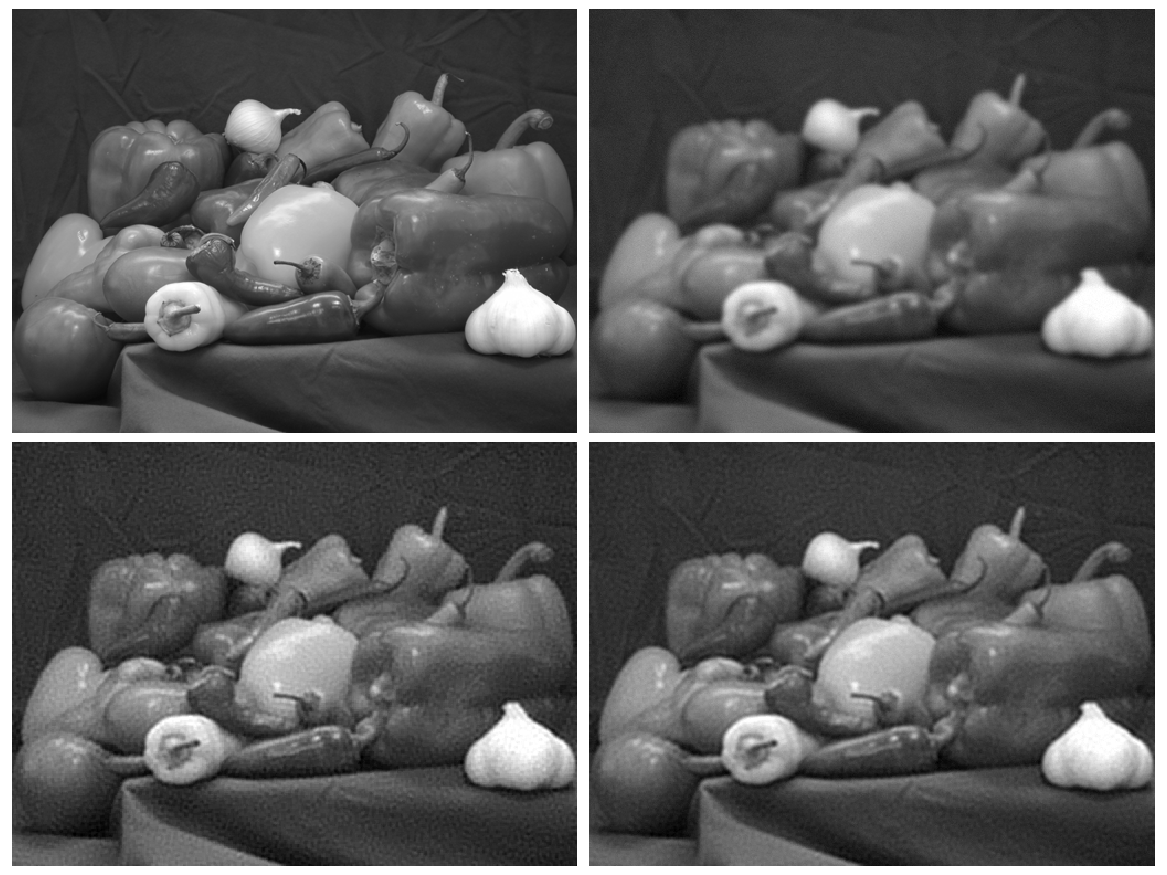
\includegraphics[width = 0.8\textwidth]{../figures/wavGaussian_2.pdf} 
\end{center}

\begin{textblock}{5}(1.5,3.6)
\rotatebox{90}{Original Image}
\end{textblock}

\begin{textblock}{5}(1.5,9.6)
\rotatebox{90}{Frobenius Loss}
\end{textblock}

\begin{textblock}{5}(14.1,3.2)
\rotatebox{90}{Blurred and Noisy}
\end{textblock}

\begin{textblock}{5}(14.1,10)
\rotatebox{90}{Huber Loss}
\end{textblock}
\end{frame}

% Results: Student's-t Noise
\begin{frame}{Results: Student's t Noise}
\begin{center}
\vspace{-3 mm}
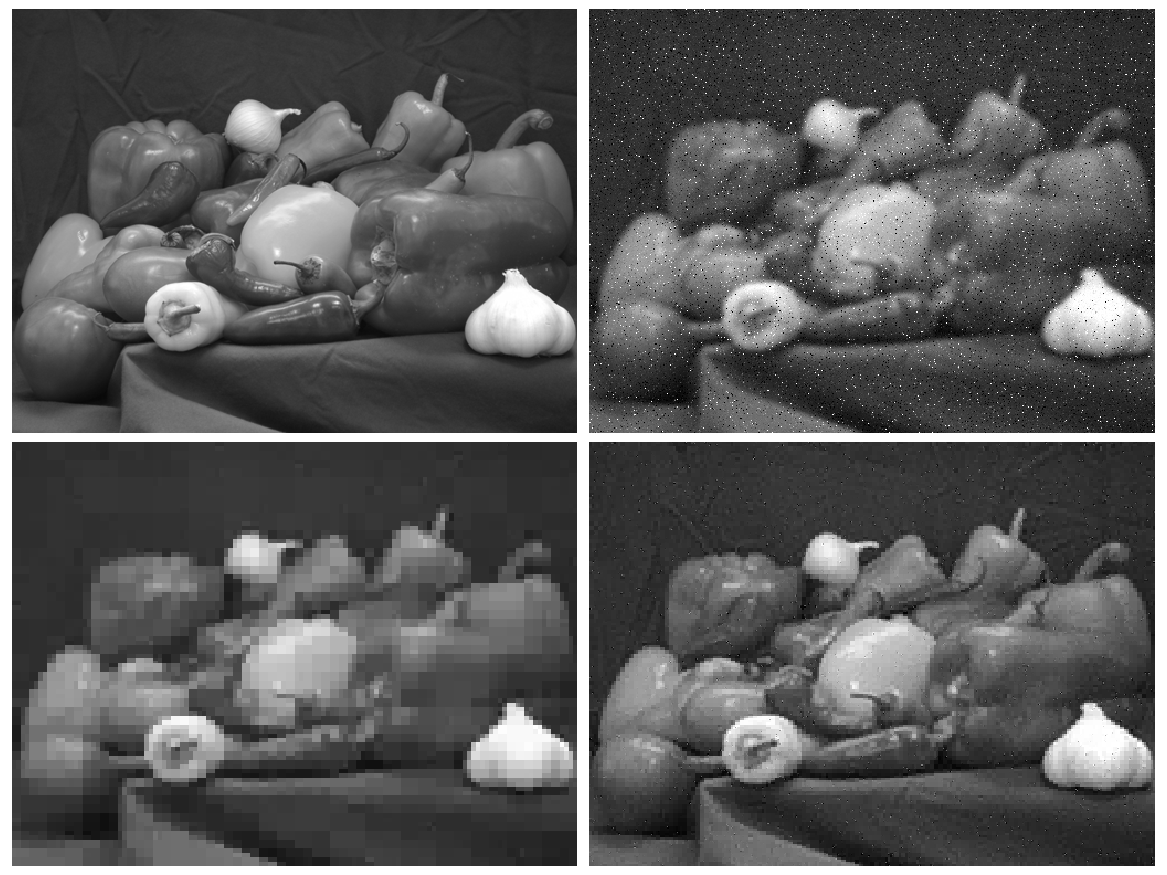
\includegraphics[width = 0.8\textwidth]{../figures/wavStudent_2.pdf} 
\end{center}

\begin{textblock}{5}(1.5,3.6)
\rotatebox{90}{Original Image}
\end{textblock}

\begin{textblock}{5}(1.5,9.6)
\rotatebox{90}{Frobenius Loss}
\end{textblock}

\begin{textblock}{5}(14.1,3.2)
\rotatebox{90}{Blurred and Noisy}
\end{textblock}

\begin{textblock}{5}(14.1,10)
\rotatebox{90}{Huber Loss}
\end{textblock}
\end{frame}

% Choosing Lambda
\begin{frame}{Choosing $\lambda$}
\begin{center}
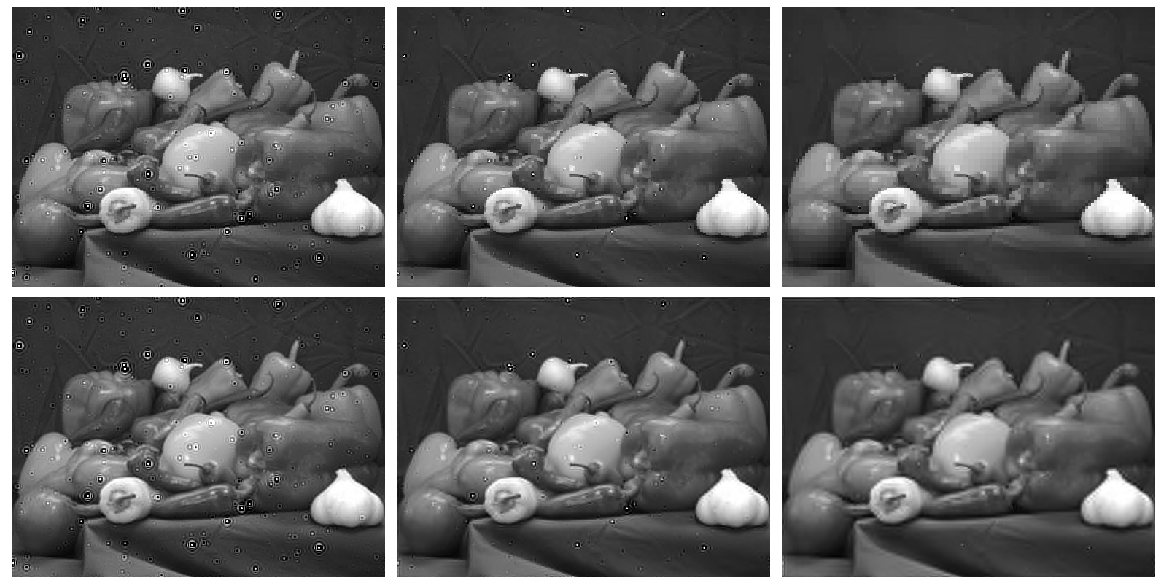
\includegraphics[width=0.9\textwidth]{../figures/wavLam.pdf}
\end{center}

\begin{textblock}{5}(0.9,6)
\rotatebox{90}{Haar}
\end{textblock}

\begin{textblock}{5}(0.9,9.5)
\rotatebox{90}{Daubechies}
\end{textblock}

\begin{textblock}{5}(2.5,13.3)
$\lambda = 10^{-4}$
\end{textblock}

\begin{textblock}{5}(6.9,13.3)
$\lambda = 10^{-3}$
\end{textblock}

\begin{textblock}{5}(11.3,13.3)
$\lambda = 10^{-2}$
\end{textblock}

\end{frame}

% OPTIMIZATION WITH TOTAL VARIATION REGULARIZATION
\section{Optimization with Total Variation Regularization}

\begin{frame}{Total Variation Regularization}

\begin{exampleblock}{Loss Function}
$$
L_b(x) = f(Ax-b) + \lambda \mathrm{TV}(x) + \delta(x | [0,1])
$$
\end{exampleblock}

\begin{exampleblock}{Proximal Gradient Step}
\begin{align*}
x^{k+1} &= \prox_{\alpha^{-1}(\lambda \|\cdot \|_{TV} + \delta_{[0,1]})} (\underbrace{x^k - \alpha^{-1} A^T\nabla f (Ax^k - b)}_{u^k}) \\
&= \AMz \left( \|u^k - z\|_F^2 + \alpha^{-1}\lambda \|z\|_{TV} + \delta(z | [0,1]) \right) \\
&= P_{[0,1]}  \left( \AMz \left( \|u^k - z\|_F^2 + \alpha^{-1}\lambda \|z\|_{TV} \right) \right)
\end{align*}
\end{exampleblock}

\end{frame}

\begin{frame}{Dual Form of Total Variation}

\begin{exampleblock}{A Few Definitions}
\begin{itemize}

\item $\mathcal{P} = \{ (p,q) \in \R^{(m-1) \times n} \times \R^{ m \times (n-1) } :  \abs{p_{i,j} } \le 1, \abs{p_{ i,j } } \le 1 \},$

\item $ \mathcal{L} : \R^{(m-1) \times n} \times \R^{ m \times (n-1) } \rightarrow \R^{m \times n}$ such that

$$ \mathcal{L}(p,q)_{i,j} = p_{i,j} + q_{i,j} - p_{ i-1,j } - q_{ i,j-1 }$$ for $i = 1,\dots,m$, $j = 1,\dots,n$, and 

$ p_{0,j} = p_{m,j} = q_{i,0} = q_{i,n} = 0.$ 

\item $P_C$ is the usual projection operator onto the set $C$

\end{itemize}
\end{exampleblock}

\begin{exampleblock}{Total Variation}
$ \mathrm{TV}(x) = max_{p,q \in \mathcal{P}} T(x, p,q) \implies T(x,p,q) = \mathrm{Tr} ( \mathcal{L}(p,q)^T x ).$
\end{exampleblock}

\end{frame}

\begin{frame}{Dual Form of TV Denoising with $\|\cdot \|_F^2$}

The problem:
$$ \min_{x \in C} \norm{x - b}_F^2 + 2 \lambda \mathrm{TV}(x), C = [0,1] $$ 
Dual problem: 
\begin{align*}
\min_{(p,q) \in \mathcal{P} } & \underbrace{- \norm{ H_C (b- \lambda \mathcal{L}(p,q) ) }_F^2 + \norm{ b - \lambda \mathcal{L}(p,q) }_F^2}_{h(p,q)} \\
H_C(x) & = \underbrace{x - P_C (x)}_{\mathrm{prox}}
\end{align*}

Optimality conditions: 

$$ x = P_C(b - \lambda \mathcal{L}(p,q) ).$$

\end{frame}

\begin{frame}{Optimization of Dual Form}

\begin{exampleblock}{Problem Statement}
\vspace{-5 mm}
\begin{align*}
&\underset{(p,q) \in \mathcal{P} }{\text{min}}  \left\{  \norm{b - \lambda \mathcal{L} (p,q)}_F^2 - \norm{(I-P_{[0,1]}) (b - \lambda \mathcal{L} (p,q))}_F^2   \right\}\\
&\underset{(p,q) }{\text{min}}  \left\{  \underbrace{\norm{b - \lambda \mathcal{L} (p,q)}_F^2 - \norm{(I-P_{[0,1]}) (b - \lambda \mathcal{L} (p,q))}_F^2}_{= h(p,q)} + \delta((p,q) | \mathcal{P})   \right\}
\end{align*}
\end{exampleblock}

\begin{exampleblock}{}
\begin{align*}
&\nabla h (p,q) = -2\lambda \mathcal{L}^TP_{[0,1]} (b - \lambda \mathcal{L}(p,q)) \\
&\text{Lipschitz with constant } \leq 16\lambda^2\\
&\Rightarrow \text{ Use projected gradient}
\end{align*}
\end{exampleblock}

\end{frame}

\begin{frame}{Optimization in Dual Form}

\begin{exampleblock}{Projection onto $\mathcal{P}$}
Recal $\mathcal{P} = (p,q) \in [-1,1]^{m-1 \times n}\times[-1,1]^{m \times n-1}$
\begin{align*}
P_\mathcal{P}(p,q) &= (r,s) \text{ with } \left\{ \begin{aligned}
r_{ij} &= sgn(p_{ij} ) \min \{ 1, |p_{ij}| \}\\
s_{ij} &= sgn(q_{ij} ) \min \{ 1, |q_{ij}| \}\\
\end{aligned}\right.
\end{align*}
\end{exampleblock}

\begin{exampleblock}{Projected Gradient Step}
\begin{align*}
(p^{k+1},q^{k+1} ) &= P_\mathcal{P} \left((p^k, q^k) + \frac{1}{8\lambda} \mathcal{L}^TP_{[0,1]} (b - \lambda \mathcal{L}(p,q)) \right)
\end{align*}
\end{exampleblock}

\end{frame}

\begin{frame}{Summary of Fast TV Regularization}
\begin{spacing}{1.6}
\fontsize{9}{10}\selectfont
\hspace{-3 mm}
\begin{minipage}{0.4\textwidth}
\textbf{MFISTA$(b,f, \lambda)$}
\begin{algorithmic}
\State $y^1 = x^0 = b; \, t^1 = 1$
\State $\alpha \geq Lip(\nabla f)$
\For {$k = 1:N$}
	\State $u^k = y^k - \frac{A^T\nabla f (A y^k - b)}{\alpha}$
	\State $z^k = FGP(u^k, \frac{\lambda}{2 \alpha})$
	\State $x^k = \underset{x \in \{x^{k-1},z^k\}}{\text{argmin}} \,L_b(x)$
	\State $t^{k+1} = \frac{1 + \sqrt{1 + 4{t^k}^2}}{2}$ 
	\State $y^{k+1} = x^k + \frac{t^k}{t^{k+1}}(z^k - x^k)$ 
	\State \hspace{10 mm}$+ \frac{t^{k-1}}{t^{k+1}}(z^k - x^k) $
\EndFor\\
\Return $x^N$
\end{algorithmic}
\end{minipage}
\begin{minipage}{0.6\textwidth}

\textbf{FGP$(b, \lambda)$}
\begin{algorithmic}
\State $(r_{ij}^1, s_{ij}^1) = (p_{ij}^0, q_{ij}^0) = 0; \, t^1 = 1$
\For {$k = 1:N$}
	\State $(p^k,q^k) = P_\mathcal{P} \left( (r^k,s^k) - \frac{\mathcal{L}^TP_{[0,1]} (b - \lambda \mathcal{L}(r^k,s^k))}{8\lambda} \right)$
	\State $t^{k+1} = \frac{1 + \sqrt{1 + 4{t^k}^2}}{2}$ 
	\State $(r^k,s^k) = (p^k,q^k) + \frac{t^k-1}{t^{k+1}}(p^k-p^{k-1}, q^k-q^{k-1})$ 
\EndFor \\
\Return $P_{[0,1]} (b - \lambda \mathcal{L}(p^N,q^N))$
\end{algorithmic}

\end{minipage}
\end{spacing}
\end{frame}

\begin{frame}{Results: Gaussian Noise}
\begin{center}
\vspace{-3 mm}
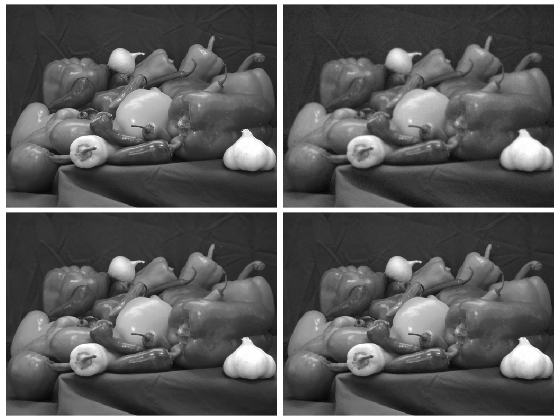
\includegraphics[width = 0.8\textwidth]{../figures/gaussian_peppers.png} 
\end{center}

\begin{textblock}{5}(1.5,3.6)
\rotatebox{90}{Original Image}
\end{textblock}

\begin{textblock}{5}(1.5,9.6)
\rotatebox{90}{Frobenius Loss}
\end{textblock}

\begin{textblock}{5}(14.1,3.2)
\rotatebox{90}{Blurred and Noisy}
\end{textblock}

\begin{textblock}{5}(14.1,10)
\rotatebox{90}{Huber Loss}
\end{textblock}

\end{frame}

\begin{frame}{Results: Student's-t Noise}
\begin{center}
\vspace{-3 mm}
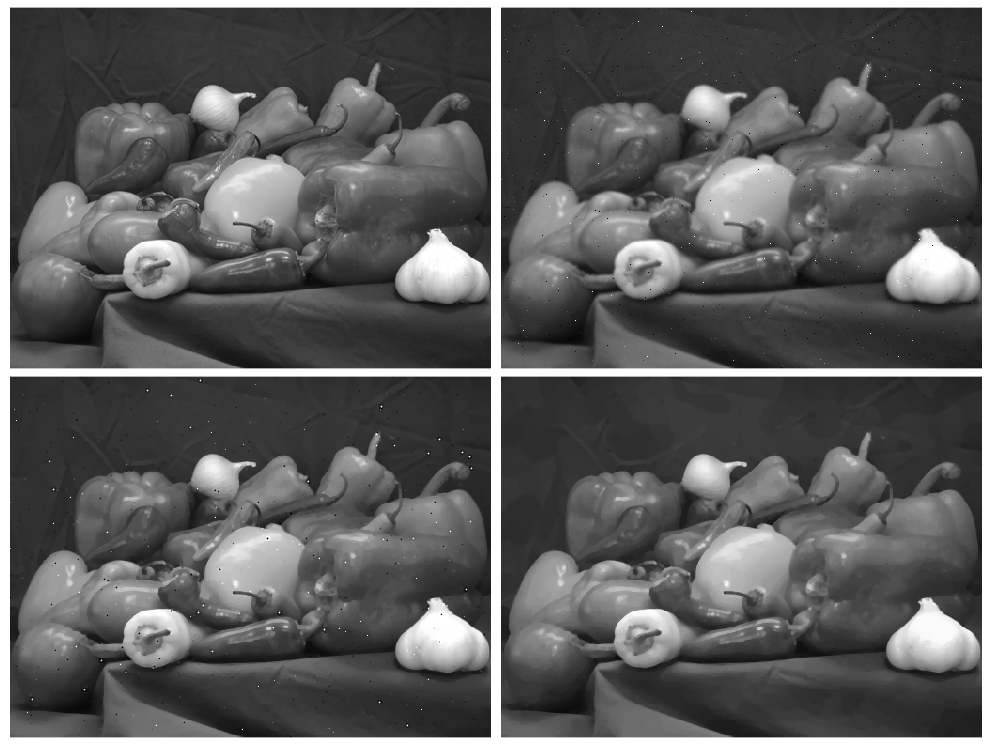
\includegraphics[width = 0.8\textwidth]{../figures/student-t_peppers.png} 
\end{center}

\begin{textblock}{5}(1.5,3.6)
\rotatebox{90}{Original Image}
\end{textblock}

\begin{textblock}{5}(1.5,9.6)
\rotatebox{90}{Frobenius Loss}
\end{textblock}

\begin{textblock}{5}(14.1,3.2)
\rotatebox{90}{Blurred and Noisy}
\end{textblock}

\begin{textblock}{5}(14.1,10)
\rotatebox{90}{Huber Loss}
\end{textblock}

\end{frame}

\section{Discussion}

\section{Discussion}

\section*{References}
\begin{frame}{Questions?}
\begin{thebibliography}{10}    
\setbeamertemplate{bibliography item}[online]
\bibitem{code} Codes used to generate figures
\url{https://github.com/snagcliffs/Amath575project}

\beamertemplatebookbibitems % This gives it a nice book symbol
\bibitem{Guck} Guckenheimer, J., Holmes, P. \textit{Nonlinear Oscillations, Dynamical Systems, and Bifurcations of Vector Fields}. Springer-Verlag, 1983. Print.

\beamertemplatearticlebibitems % and an article symbol
\bibitem{brazil}  Oliveira, D., Leonel, E. (2008) \textit{Braz. J. Phys.} 38(1):62-64

\bibitem{corrdim} Grassberger, P., Procaccia, I. (1983) \textit{Phys. Rev. Letters.} 50(5):346-349

\end{thebibliography}
\end{frame}

\end{document}
